\section{Calendari}
La gestione dei calendari è accessibile mediante apposito menù come in figura
\ref{fig:amministratore_menu_generale_selezione_calendari.pdf}
\begin{figure}[H]
\centering{}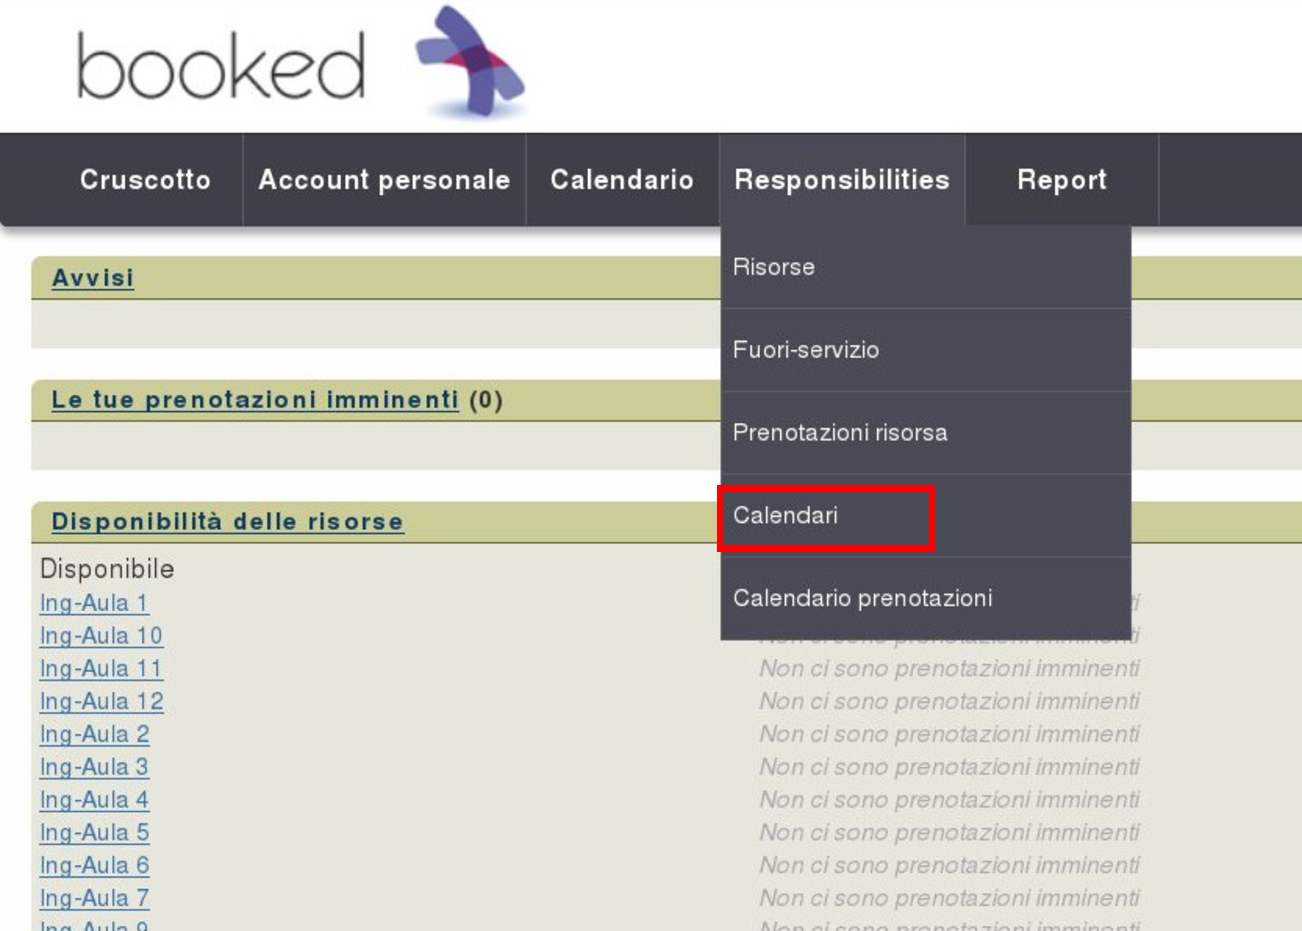
\includegraphics[scale=0.5]{Immagini/amministratore_menu_generale_selezione_calendari.pdf}
\normalsize
\caption{}
\label{fig:amministratore_menu_generale_selezione_calendari.pdf}
\end{figure}

all'interno è possibile gestire le fasce orarie disponibili, ed il frazionamento degli intervalli orari.
Non confondere la gestione calendari con la gestione delle prenotazioni, che si fa altrove.
Dopo la creazione di un nuovo calendario, accedere all'opzione ``cambia layout'' e controllare che il fuso
orario sia Europe/Rome.